\documentclass[border=4pt]{standalone}

\usepackage{amsmath}
\usepackage{tikz}
\usepackage{mathdots}
\usepackage{yhmath}
\usepackage{cancel}
\usepackage{color}
\usepackage{siunitx}
\usepackage{array}
\usepackage{multirow}
\usepackage{amssymb}
\usepackage{gensymb}
\usepackage{tabularx}
\usepackage{booktabs}
\usetikzlibrary{fadings}
\usetikzlibrary{patterns}


\begin{document}

\tikzset{every picture/.style={line width=0.75pt}} %set default line width to 0.75pt        

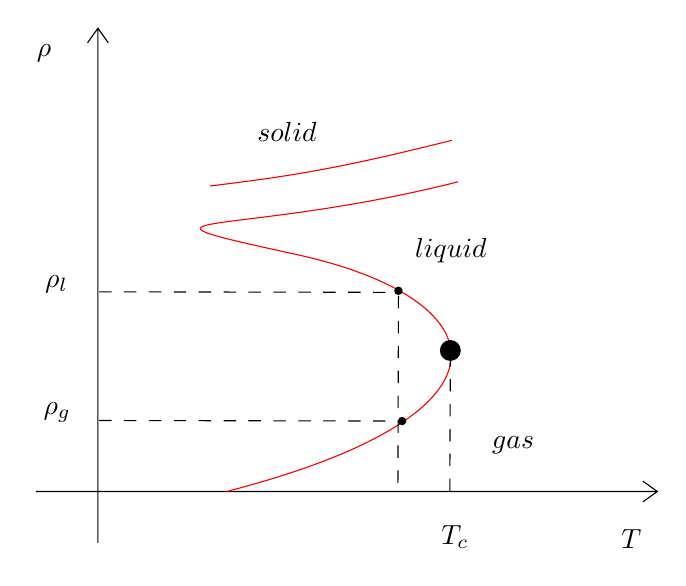
\begin{tikzpicture}[x=0.75pt,y=0.75pt,yscale=-1,xscale=1]
%uncomment if require: \path (0,300); %set diagram left start at 0, and has height of 300

%Shape: Axis 2D [id:dp5838325963013411] 
\draw  (50,236.2) -- (349.5,236.2)(79.95,13) -- (79.95,261) (342.5,231.2) -- (349.5,236.2) -- (342.5,241.2) (74.95,20) -- (79.95,13) -- (84.95,20)  ;
%Curve Lines [id:da4435327399422857] 
\draw [color={rgb, 255:red, 255; green, 0; blue, 0 }  ,draw opacity=1 ]   (253.5,87) .. controls (146.5,114) and (79.5,101) .. (175.5,122) .. controls (271.5,143) and (289.5,198) .. (141.95,236.2) ;


%Shape: Circle [id:dp6950646185312648] 
\draw  [fill={rgb, 255:red, 0; green, 0; blue, 0 }  ,fill opacity=1 ] (254.5,168.25) .. controls (254.5,165.63) and (252.37,163.5) .. (249.75,163.5) .. controls (247.13,163.5) and (245,165.63) .. (245,168.25) .. controls (245,170.87) and (247.13,173) .. (249.75,173) .. controls (252.37,173) and (254.5,170.87) .. (254.5,168.25) -- cycle ;
%Straight Lines [id:da310151440009067] 
\draw  [dash pattern={on 4.5pt off 4.5pt}]  (80.5,140) -- (224.75,140.25) ;


%Straight Lines [id:da9372276877276311] 
\draw  [dash pattern={on 4.5pt off 4.5pt}]  (80.5,202) -- (224.75,202.25) ;


%Shape: Circle [id:dp7624553374051801] 
\draw  [fill={rgb, 255:red, 0; green, 0; blue, 0 }  ,fill opacity=1 ] (226.5,139.5) .. controls (226.5,138.53) and (225.72,137.75) .. (224.75,137.75) .. controls (223.78,137.75) and (223,138.53) .. (223,139.5) .. controls (223,140.47) and (223.78,141.25) .. (224.75,141.25) .. controls (225.72,141.25) and (226.5,140.47) .. (226.5,139.5) -- cycle ;
%Shape: Circle [id:dp5614900522339243] 
\draw  [fill={rgb, 255:red, 0; green, 0; blue, 0 }  ,fill opacity=1 ] (228.25,202.25) .. controls (228.25,201.28) and (227.47,200.5) .. (226.5,200.5) .. controls (225.53,200.5) and (224.75,201.28) .. (224.75,202.25) .. controls (224.75,203.22) and (225.53,204) .. (226.5,204) .. controls (227.47,204) and (228.25,203.22) .. (228.25,202.25) -- cycle ;
%Straight Lines [id:da025024757163219613] 
\draw  [dash pattern={on 4.5pt off 4.5pt}]  (224.5,232) -- (224.75,141.25) ;


%Straight Lines [id:da7521958610536339] 
\draw  [dash pattern={on 4.5pt off 4.5pt}]  (249.5,236) -- (249.75,168.25) ;


%Curve Lines [id:da8707463865980332] 
\draw [color={rgb, 255:red, 255; green, 0; blue, 0 }  ,draw opacity=1 ]   (134,89) .. controls (175.5,84) and (198.5,80) .. (250.5,67) ;



% Text Node
\draw (54,25) node   {$\rho $};
% Text Node
\draw (337,259) node   {$T$};
% Text Node
\draw (60,136.33) node   {$\rho _{l}$};
% Text Node
\draw (60.33,198) node   {$\rho _{g}$};
% Text Node
\draw (252,258) node   {$T_{c}$};
% Text Node
\draw (280,214) node   {$gas$};
% Text Node
\draw (250,120) node   {$liquid$};
% Text Node
\draw (171,63) node   {$solid$};


\end{tikzpicture}
\end{document}
